\documentclass{standalone}
\usepackage{tikz}
\usepackage{amsmath}

\begin{document}

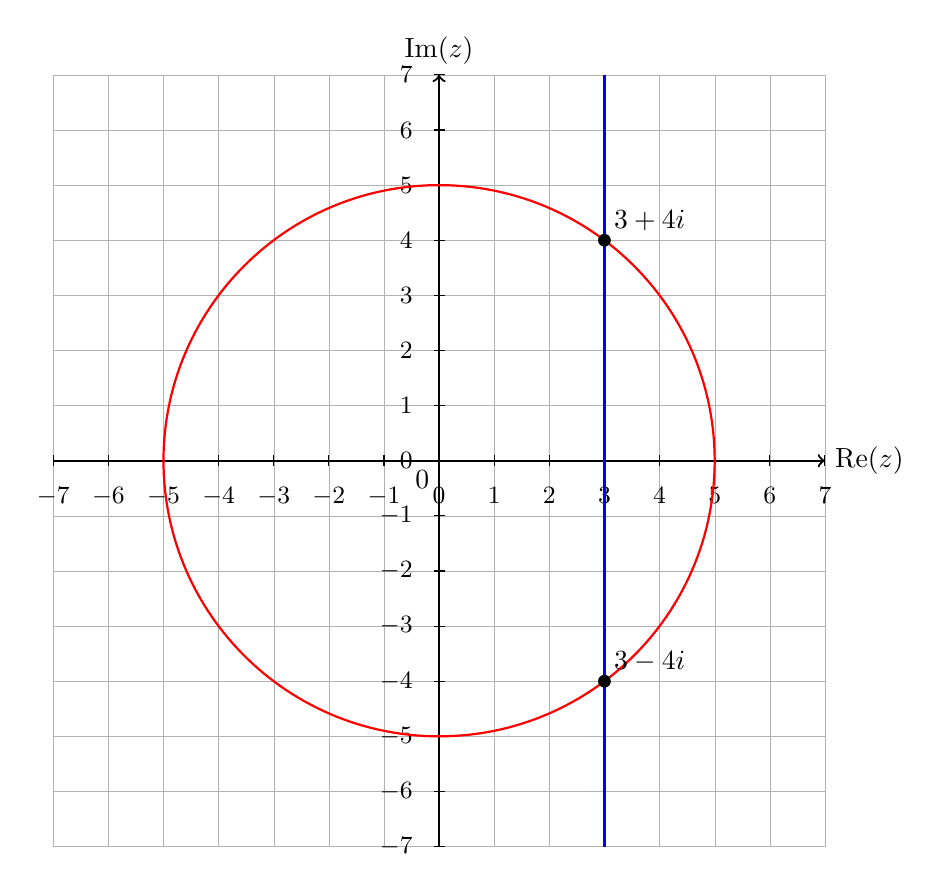
\begin{tikzpicture}[scale=.7]
    
    % Center of the circle
    \def\xmin{-7}
    \def\xmax{7}
    \def\ymin{-7}
    \def\ymax{7}
    \def\dxthick{2}
    \def\dythick{2}
    \def\dx{.5}
    \def\dy{.5}
    \def\xminb{\xmin-\dx}
    \def\xmaxb{\xmax+\dx}
    \def\yminb{\ymin-\dy}
    \def\ymaxb{\ymax+\dy}

%   % Fill outside region
%   \begin{scope}
%       \clip (\xminb, \yminb) rectangle (\xmaxb, \ymaxb);
%       \fill[gray!30] (\xmin, \ymin) rectangle (\xmax, \ymax);
%       \fill[white] (center) circle (2);
%   \end{scope}

    % Draw grid
    \draw[step=1., gray!60, ultra thin] (\xmin, \ymin) grid (\xmax, \ymax); % Visible grid with lighter color
    
    % Axes
    \draw[->, thick] (\xmin, 0) -- (\xmax, 0) node[right] {$\text{Re}(z)$};
    \draw[->, thick] (0, \ymin) -- (0, \ymax) node[above] {$\text{Im}(z)$};

    % Axis ticks
    \foreach \x in {\xmin,..., \xmax}
        \draw (\x, -0.1) -- (\x, 0.1) node[below=8pt] {\small $\x$};
    \foreach \y in {\ymin,..., \ymax}
        \draw (-0.1, \y) -- (0.1, \y) node[left=8pt] {\small $\y$};

    % Labels for axes
    \node[below left] at (0, 0) {$0$};

    % Line
    \draw[blue, thick] (3, \ymin) -- (3, \ymax); % node[right] {$\text{Re}(z)$};
    
    % Circle
    \coordinate (center) at (0., 0.);
    \draw[red, thick] (center) circle (5);
    
    % Solutions
    \coordinate (z1) at (3, 4);
    \coordinate (z2) at (3,-4);
    \filldraw[black] (z1) circle (3pt) node[above right] {$3+4i$};
    \filldraw[black] (z2) circle (3pt) node[above right] {$3-4i$};
%
%   % Radius line
%   \draw[dashed] (center) -- ++(2, 0) node[midway, below] {$r = \radius$};
        
\end{tikzpicture}

\end{document}
